\section{Umsetzungskonzept}
Die Grundidee für die Umsetzung der Fussgängerstreifen Erkennung lässt sich in folgenden Punkten zusammenfassen:
\begin{enumerate}
	\item Download der Strassen- und Fussgängerstreifenkoordinaten
	\item Download von Orthofotos auf \Gls{OpenStreetMap} Zoomlevel 19
	\item Anfertigen von einheitlichen Bildern entlang der Strassen
	\item Fussgängerstreifenerkennung mithilfe des Convnets
	\item Vergleich bestehende Fussgängerstreifen mit neu gefundenen
	\item Parallelisierung des Erkennungsprozesses
	\item Daten in eine Maproulette Challenge umwandeln
\end{enumerate}


\subsection{OpenStreetMap Anbindung}
Um Daten von OpenStreetMap zu erhalten, kann man eine OpenStreetMap Web API ansprechen. Mapquest\footnote{\url{http://open.mapquestapi.com/xapi/}} stellt eine solche OpenStreetMap API zur Verfügung. Mit dieser Schnittstelle lassen sich via HTTP GET Abfragen starten. Eine Bounding Box und die entsprechenden OpenStreetMap Tags dienen als Input. Man erhält danach alle Daten in einem einfach zu interpretierenden XML Format. Mit der gleichen Abfrage lassen sich sogar Fussgängerstreifen und Strassen gleichzeitig herunterladen.

\begin{figure}[H]
	\centering
	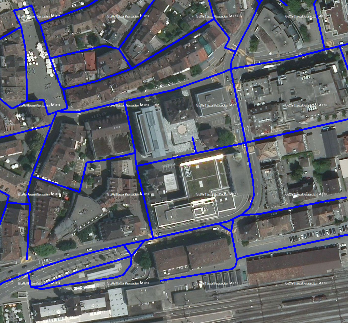
\includegraphics{images/Strassen_Rapperswil.png}
	\caption{Eingezeichnete Strassen in Rapperswil}
\end{figure}

\newpage
\subsection{Bing Anbindung}
Um an die Orthofotos zu kommen, gab es zu Beginn des Projektes mehrere Lösungen:
\begin{enumerate}
	\item Offizielle Microsoft Bing REST Service
	\item Direkter Download über Bing Maps
	\item Benutzung der Orthofotos von der HSR
\end{enumerate}

Als aller erstes haben wir versucht, die Orthosfotos über den offizielle Microsoft Bing REST Service\footnote{\url{https://msdn.microsoft.com/en-us/library/ff701713.aspx}} zu download. Jedoch beschränkt Microsoft den API Zugriff auf 50'000 Transaktionen pro Tag und 125'000 Transaktionen pro Jahr, was uns bei geschätzten 7 Millionen Tiles in der Schweiz nicht reichen würde.

Nachdem diesem ersten Versuch sind wir auf den direkten Download der Othosfotos umgestiegen. Wenn man mit dem Internet Browser auf Bing Maps zugreift, werden die \Gls{Tile}s mithilfe von Javascript von den Bing Servern geladen. Microsoft benutzt das Quadtree\footnote{\url{https://msdn.microsoft.com/en-us/library/bb259689.aspx}} Format, um die entsprechenden Tiles anzusprechen. Mithilfe des Projekts Tiles à la Google Maps\footnote{\url{http://www.maptiler.org/google-maps-coordinates-tile-bounds-projection/}} und der dort zur Verfügung gestellten Python Library, können wir Bounding Boxen in Quadtrees umwandeln.

Die Orthofotos, welche im Besitz der HSR sind und die nur die Schweiz umfassen, wären die letzte Lösung gewesen, wenn die anderen Möglichkeiten versagt hätten.
\subsection{Convolutional Neural Network}
Die Evaluation des Suchalgorithmus hat einen klaren Sieger ergeben. Das Convolutional\footnote{Convolutional ist Englisch und heisst auf Deutsch Faltung} Neural Network (hier weiter als Convnet bezeichnet) liefert mit Abstand die besten Resultate innerhalb unserer Test Bounding Box in Rapperswil.

\subsubsection{Geschichte}
Bis noch vor einigen Jahren wurden neuronale Netze zur Bilderkennung grösstenteils ignoriert\footnote{\url{http://karpathy.github.io/2015/10/25/selfie/}}. Das Convnet selbst wurde schon 1980 von einem Japaner namens Fukushima erfunden, jedoch erhielt es keine grössere Beachtung. Hauptgrund dafür war der Rechenhunger für das Training des Netzes. Gedreht hat sich das Ganze erst als 2012 genügend Rechenleistung mithilfe von Grafikkarten zur Verfügung stand. Ab diesem Zeitpunkt erzielte diese wieder gefundene Technik Bestleistungen in vielen Bereichen der Bilderkennung. Bis heute ist das Convnet die präziseste Technik zur Erkennung von Gegenständen in Fotos.

\subsubsection{Funktionsweise}
Ein künstliches neuronales Netz besteht aus einer grossen Anzahl von simulierten Neuronen. Mit verschiedenen Techniken aus der Statistik und  Mathematik kann so ein Input auf einen Output gemappt werden. In unserem Fall wollen wir ein Bild auf eine der Kategorien Crosswalk oder Non-Crosswalk mappen. Dies wird in der Fachliteratur auch Klassifikation von Bildern genannt.

Wie der Name schon sagt, besteht das Convolutional Neuronale Netz aus vielen verschiedenen Faltungsfilter. Ein Faltungsfilter transformiert ein Bild so, dass ein spezifisches Muster auf dem Bild markiert wird. Ein gutes Beispiel für einen Filter ist die Technik der Kantendetektion\footnote{\url{https://de.wikipedia.org/wiki/Kantendetektion}}. Die Kantendetektion markiert nur die Kanten auf dem Bild und ignoriert den restlichen Inhalt.\\

\begin{figure}[H]
	\centering
	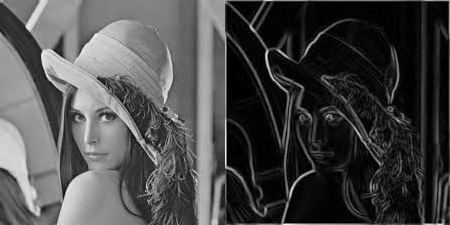
\includegraphics{images/kantendetektion.jpg}
	\caption{Beispiel einer Kantendetektion}
\end{figure}
Ein Convolutional Neuronales Netz lernt nun selbst, welchen Faltungsfilter er anwendet, um das Problem möglichst gut zu lösen. Die extrahierten Muster dienen als Features und werden nun von einem einfachen Neuronalen Netz klassifiziert. Die Ausgabe besteht nun aus aus zwei Werten zwischen 0 und 1. Sie stellen die Wahrscheinlichkeiten der entsprechenden Klasse dar.

\subsubsection{Keras}
Das Projekt Keras\footnote{\url{https://github.com/fchollet/keras}} stellt eine einfache Library zum Entwerfen und Trainieren von Neuronalen Netzen zur Verfügung. Es bietet modulare Funktionen für Convolutional Neuronale Netzwerke und Rekurrente Netzwerke an. Mithilfe eines Flags kann das Training einfach auf die Grafikkarte ausgelagert werden, was bei solchen Algorithmen unerlässlich ist.
\newpage
\section{Parallelisierung}
Zu Beginn unserer Arbeit unterschätzten wir die enorme Datenmenge in Form von Orthofotos (Beispiel Schweiz: 7.1 Millionen Bilder à $5820 m^{2}$ Fläche pro Bild). Weiter wird auch sehr viel Rechenleistung für die Erkennung der Fussgängerstreifen auf den Bilder benötigt. Um diesen nicht trivialen Problemen Herr zu werden, setzten wir auf eine Parallelisierungsstratege mit Hilfe einer Queue. \\ 

\decision{Queueing Sytem}
Den Entscheid für Redis\footnote{\url{http://redis.io/}} in Kombination mit RQ\footnote{\url{http://python-rq.org/}} haben wir während eines Meeting mit Hilfe von Mitarbeitern des Institut für Software erarbeitet. RQ ist eine relativ einfach zu verwendende Library, welche Redis (Key Value Store) als Queue einsetzt. Durch die Einfachheit und die gute Integration in Python haben wir uns für diesen Lösungsweg entschieden.

\newpage
\subsection{Ablauf}
\label{subsec:ablauf}
\begin{figure}[H]
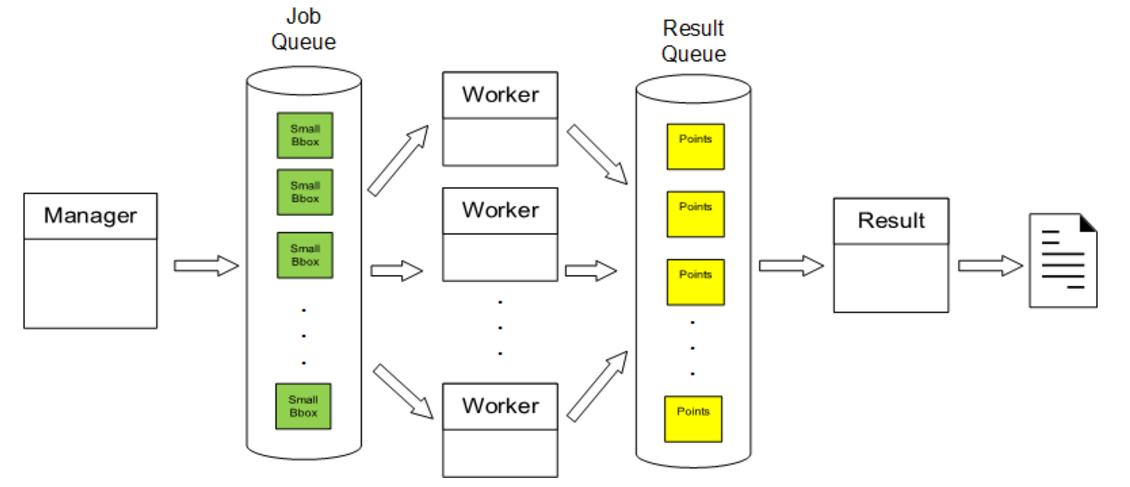
\includegraphics[width=\textwidth]{images/queuing.png}
\caption[Queueing]{Queueing}
\end{figure}
Auf der Abbildung ist zu sehen, dass wir für das Verarbeiten der Jobs auf zwei Queues setzten, eine die die Abzuarbeitenden Bounding Boxes beinhaltet und eine weitere für das Sammeln der Resultate. Der genau Ablauf gestaltet sich wie folgt:
\begin{enumerate}
		\item Manager wird aufgerufen mit der grosse Input Bounding Box.
		\item Manager teilt Bounding Box auf.
		\item Kleine Bounding Boxes werden als Jobs in die Job Queue geladen.
		\item Jobs werden von den Worker aus der Queue geholt.
		\item Worker arbeiten kleine Bounding Boxen ab.
		\item Worker stellt die gefunden Punkt in Result Queue.
		\item Result Worker holt die gefunden Punkt aus der Result Queue und speichert diese in einer JSON Datei ab. 
\end{enumerate}










\subsection{MapRoulette}
Maproulette ist ein Crowdsourcing-System, welches genutzt wird um mit Hilfe von Challenges Daten in OpenStreetMap einfliessen zu lassen, diese kontrolliert oder auch erweitert. Den Entscheid für diesen Anbieter haben wir unter dem Abschnitt~\ref{subsec:MapRoulette} auf der Seite~\pageref{subsec:MapRoulette} getroffen.

\subsubsection{Daten in Tasks umwandeln}
Am Ende des Suchprozesses werden alle gefundenen Fussgängerstreifen in einer JSON Datei abgespeichert. MapRoulette benötigt für die Tasks jedoch ein GeoJSON Format, somit mussten wir diese Daten noch passend umwandeln. 

\paragraph{Challenge} Der Text für die Challenge ist in englisch zu verfassen und sollte folgende Punkte beinhalten:
\begin{itemize}
	\item Title
	\item Blurb (Einzeiler, eine Art Untertitel)
	\item Description
	\item Help
	\item Instruction
\end{itemize}

\paragraph{Task} Unsere Task beinhalte hauptsächlich nur die Position des zu verifizierenden Fussgängerstreifens, sowie eine kurze Beschreibung. Der Aufbau gliedert sich folgendermassen:
\begin{itemize}
	\item Identifier (Eindeutiger 72 Character String)
	\item Geometries (Position des Fussgängerstreifens)
	\item Instruction (Beschriebt den Task)
\end{itemize}

